 
\usetheme{LUH}


\unitlength1cm
% \renewcommand{\parnoteintercmd}{\penalty-1000\hskip 1em plus 10em minus 0.2em}
\makeatletter
\global\def\bibli@finale{}
\newcommand{\parcite}[2][]{\parnote{#1\fullcite{#2}}
    \unless\ifx\bibli@finale\@empty\g@addto@macro\bibli@finale{\parnoteintercmd}\fi
    % Redefine \@currentlabel to the parnote label, so \label works
    \g@addto@macro\bibli@finale{\phantomsection\def\@currentlabel{#1}}%
    \g@addto@macro\bibli@finale{\cite{#2}}%
}
\newcommand{\bibliographie}{\setbox0=\hbox{\bibli@finale}
\printbibliography}
\makeatother

% macro vim pour transformer des points en centimètres: d:r!echo <c-r>"/28.4 | bc -lq<c-m>vEdu<c-r>PjJ
\setbeamertemplate{logonortheastp1}{\begin{picture}(0,0)(0,0)
\put(-0,-1.056){\llap{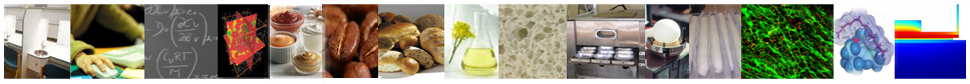
\includegraphics[width=.95\textwidth]{hautp1.png}}}\end{picture}}
\setbeamertemplate{logonorthwestp1}{}
\setbeamertemplate{logosoutheastp1}{\begin{picture}(0,0)(.70422535211267605633,.07042253521126760563)
\put(0,.70422535211267605633){\llap{

\includegraphics[height=1cm]{logoAPT.png}%

\includegraphics[height=1cm]{logoINRA.png}}}~
\end{picture}
}
\setbeamertemplate{logosouthwestp1}{\begin{picture}(0,0)(-.17605633802816901408,-.03521126760563380281)
\put(1.76056338028169014084,0){\llap{
\includegraphics[height=19mm]{coinbasgauche.jpg}}}
\put(.42253521126760563380,1.86619718309859154929){
\includegraphics[height=.93\textheight]{traitgauche.png}}
\put(1.58450704225352112676,.21126760563380281690){

\includegraphics[width=.88\textwidth]{traitbas.png}}
\put(.70422535211267605633,1.12676056338028169014){\color{red}Ingénierie Procédés Aliments}
\put(.70422535211267605633,.77464788732394366197){\color{red}\textit{(Food \& Process Engineering)}}
\end{picture}
}
% \titleimage{\includegraphics[width=.7\paperwidth]{luh_title_image}}
\setbeamertemplate{logonortheast}{\begin{picture}(0,0)(0,0)
\put(0,-.70422535211267605633){\llap{
\includegraphics[width=.94\textwidth]{haut.png}}}
\end{picture}}
\setbeamertemplate{logosouthwest}{\begin{picture}(0,0)(-.17605633802816901408,-.03521126760563380281)
\put(1.76056338028169014084,0){\llap{
\includegraphics[height=19mm]{coinbasgauche.jpg}}}
\put(1.58450704225352112676,.21126760563380281690){

\includegraphics[width=.88\textwidth]{traitbas.png}}
\put(-.17605633802816901408,1.86619718309859154929){\rotatebox{90}{\rlap{

\includegraphics[height=5mm]{logoAPT.png}%

\includegraphics[height=5mm]{logoINRA.png}}}}
\put(.42253521126760563380,1.86619718309859154929){
\includegraphics[height=.93\textheight]{traitgauche.png}}
\end{picture}
}
% \setbeamertemplate{logosoutheast}{
\includegraphics[height=\LUHLogoHeight]{traitbas.png}}

\AtBeginSection[]% merci http://jeromyanglim.tumblr.com/post/33559584570/how-to-show-active-section-in-table-of-contents-in
{
   \begin{frame}
       \tableofcontents[currentsection]
   \end{frame}
}

% \usepackage[para]{footepackage{parnotes}% marche pas dans beamer.
